Introduction \cite{huff_extensions_2014}.

\section{Micro Reactors}

Microreactors have three main features: Factory fabricated, transportable, and self-regulating. All components of a microreactor would be fully assembled in a factory and shipped out to location. This feature reduces capital costs and would allow to deploy the reactor quickly. Smaller unit designs will make the reactors easy to transport, requiring less installation time. Simple design concepts will eliminate the need of a large number of specialized operators. They would utilize passive safey systems that prevent any potential of overheating or meltdown.

Most of the microreactor designs vary, but most would be able to produce 1-20 MW of thermal energy. The microreactor could serve several purposes among which are electric power production or heat production for district heating, water desalination, and hydrogen fuel production.
\cite{noauthor_ultimate_2019}.

Microreactor designs will alow island-mode operations, black-start capabilities, an ability to protect against severe natural phenomena as well as man-made physical and cyber security threats, and to operate for several years without the need to shutdown for refueling \cite{nichol_roadmap_2018}.

MMR's can produce industrial process steam, industrial heat, desalination, greenhouses, aqua farms, and district heating.

\section{High Temperature Gas-cooled systems}

The high-temperature gas-cooled reactor concept benefits from the development of high-temperature reactors from 1970 to 1980 in the United States, France, Germany, and the United Kingdom. 
Among its advantages are:
- Achievement of higher temperatures (1000 C): This will improve electrical production efficiency by up to 50\%. This increase in coolant temperature would also enable efficient hydrogen production.
- Helium as coolant. It is chemicall neutral, it is nearly transparent to neutrons, and does not become radioactive.
- The fuel provides excellent confinement of the fission products. Very low particle failure rate up to 1800$^{\circ}$C. High burn-up capability, in experiments burn-ups of 780GWd/t without damage of the particles.
- Past experiences: Fort St-Vrain (US), HTTR (Japan), and HTR-10 (China).
\cite{france_gas-cooled_2006}

\section{MMR - USNC}

The Micro Modular Reactor (MMR) concept integrates power production, power conversion, and electricity generation in a single unit, making it suitable for use in remote areas. 
The MMR will use hexagonal graphite blocks containing stacks of fully ceramic micro-encapsulated (FCM) fuel, which is a form of TRISO fuel, and He (or CO$_2$) as coolant.
The power of this reactor will range between 10 to 40 MW-thermal and its cycle length will be greater than 20 years.
The MMR design results attractive for replacing diesel generators in remote areas. As it could be factory produced, it could generate power at economically competitive prices \cite{hawari_development_2018}.

\begin{figure}[H]
	\centering
	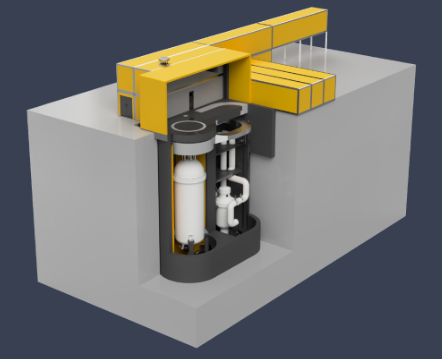
\includegraphics[width=0.5\linewidth]{figures/mmr.png}
	\hfill
	\caption{MMR nuclear plant \cite{usnc_mmr_2019}.}
	\label{fig:triso}
\end{figure}

\section{FCM}

FCM fuel is stable under irradiation and capable of withstanding temperatures well in excess of all postulated accident conditions, ensuring total contaiment of radioactivity \cite{usnc_mmr_2019}.

The fuel compact is 0.7 cm radius, and it could vary from 0.4 to 0.7 cm \cite{powers_fully_2013}. The fuel compact contains the TRISO particles in Carbide compact (SiC), and the packing fraction determines the number of particles in the fuel. The packing fraction ranges from 40 to 58\% \cite{powers_fully_2013}. The model assumes a 40\% packing fraction.

\subsection{TRISO particles}

A typical TRISO particle has a kernel and 4 layers Fig. \ref{fig:triso}. The kernel has the fissile material (UO$_2$, UCO, UN, etc.). The layers (from the inside to the outside) are buffer, inner pyrolytic carbon (IPyC), silicon carbide (SiC), and outer pyrolytic carbon (OPyC).
The model assumes a kernel of UN with a 700 $\mu$m-diameter. The layers have a thickness of 50, 35, 35, and 20 $\mu$m, respectively.
The density for the kernel is 14.32 g/cc and for the layers it is 1.05, 1.9, 3.18, 1.9 g/cc, respectively. The enrichment is 12\%. For the SiC, the layer has a Si weight fraction of 70.05\% while the rest is Graphite. The rest of the layers only component is Graphite.

\begin{figure}[H]
	\centering
	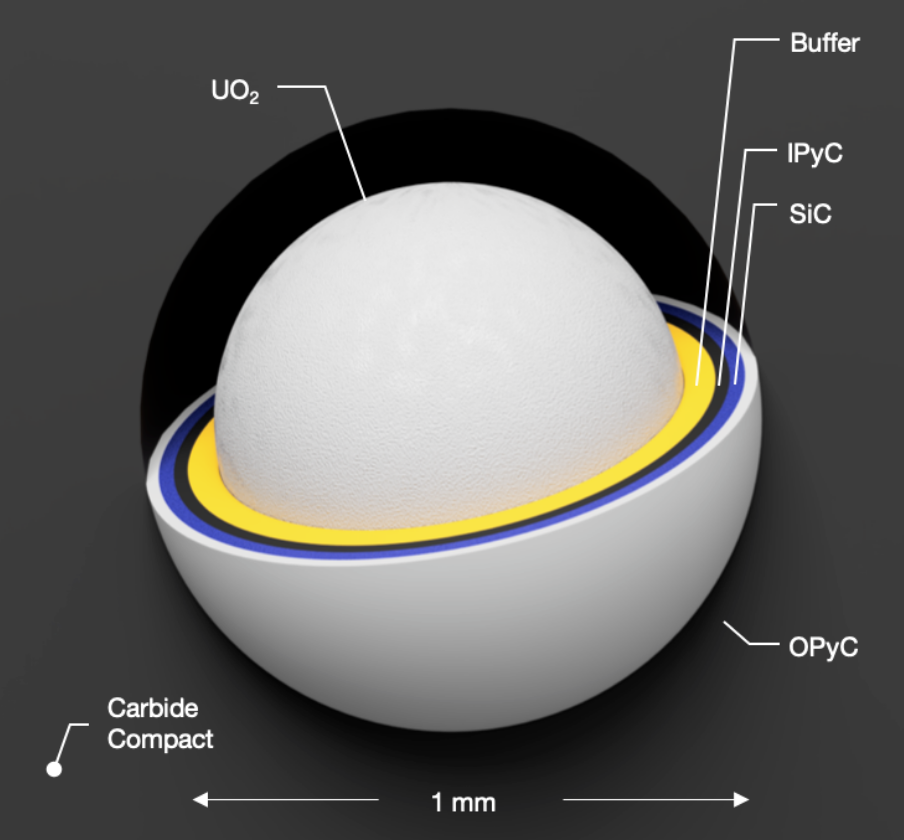
\includegraphics[width=0.5\linewidth]{figures/triso1.png}
	\hfill
	\caption{Typical TRISO particle [Add reference to the website].}
	\label{fig:triso}
\end{figure}

Buffer layer of porous carbon serving as a reservoir for fission gases.
Layers of dense pyrolytic carbon contribute to the mechanical resistance of the particle.
The silicon carbide layer serves as a fission product diffusion barrier.
\cite{france_gas-cooled_2006}